\documentclass{scrartcl}

\usepackage[usenames,dvipsnames,svgnames]{xcolor}
\usepackage[shortlabels]{enumitem}
\usepackage[framemethod=TikZ]{mdframed}
\usepackage{amsmath,amssymb,amsthm}
\usepackage{epigraph}
\usepackage[colorlinks]{hyperref}
\usepackage{microtype}
\usepackage{mathtools}
\usepackage[headsepline]{scrlayer-scrpage}
\usepackage{thmtools}
\renewcommand{\epigraphsize}{\scriptsize}
\renewcommand{\epigraphwidth}{60ex}
\addtolength{\textheight}{3.14cm}
\ihead{\footnotesize\textbf{Junior Math Team Notes}}
\ohead{\footnotesize \today}
\providecommand{\clubs}[1]{$#1\clubsuit$}
\providecommand{\ol}{\overline}
\providecommand{\eps}{\varepsilon}
\providecommand{\half}{\frac{1}{2}}
\providecommand{\dang}{\measuredangle} %% Directed angle
\providecommand{\CC}{\mathbb C}
\providecommand{\FF}{\mathbb F}
\providecommand{\NN}{\mathbb N}
\providecommand{\QQ}{\mathbb Q}
\providecommand{\RR}{\mathbb R}
\providecommand{\ZZ}{\mathbb Z}
\providecommand{\dg}{^\circ}
\providecommand{\ii}{\item}
\providecommand{\alert}{\textbf}
% hacks for arc
\providecommand{\tarc}{\mbox{\large$\frown$}}
\providecommand{\arc}[1]{\stackrel{\tarc}{#1}}
\reversemarginpar
\providecommand{\printpuid}[1]{\marginpar{\href{https://otis.evanchen.cc/arch/#1}{\ttfamily\footnotesize\color{green!40!black}#1}}}

\mdfdefinestyle{mdbluebox}{roundcorner=10pt,innerbottommargin=9pt,
	linecolor=blue,backgroundcolor=TealBlue!5,}
\declaretheoremstyle[headfont=\sffamily\bfseries\color{MidnightBlue},
mdframed={style=mdbluebox},]{thmbluebox}

\mdfdefinestyle{mdredbox}{frametitlefont=\bfseries,innerbottommargin=8pt,
	nobreak=true,backgroundcolor=Salmon!5,linecolor=RawSienna,}
\declaretheoremstyle[headfont=\bfseries\color{RawSienna},
mdframed={style=mdredbox},headpunct={\\[3pt]},postheadspace=0pt,]{thmredbox}

\mdfdefinestyle{mdgreenbox}{linecolor=ForestGreen,backgroundcolor=ForestGreen!5,
	linewidth=2pt,rightline=false,leftline=true,topline=false,bottomline=false,}
\declaretheoremstyle[headfont=\bfseries\sffamily\color{ForestGreen!70!black},
mdframed={style=mdgreenbox},headpunct={ --- },]{thmgreenbox}

\mdfdefinestyle{mdorangebox}{linecolor=RedOrange,backgroundcolor=RedOrange!5,
	linewidth=2pt,rightline=false,leftline=true,topline=false,bottomline=false,}
\declaretheoremstyle[headfont=\bfseries\sffamily\color{RedOrange!70!black},
mdframed={style=mdorangebox},headpunct={ --- },]{thmorangebox}

\mdfdefinestyle{mdblackbox}{linecolor=black,backgroundcolor=RedViolet!5!gray!5,
	linewidth=3pt,rightline=false,leftline=true,topline=false,bottomline=false,}
\declaretheoremstyle[mdframed={style=mdblackbox}]{thmblackbox}

\declaretheorem[style=thmredbox,name=Problem,numberwithin=section]{problem}
\declaretheorem[style=thmredbox,name=Required Problem,sibling=problem]{reqproblem}
\declaretheorem[style=thmbluebox,name=Theorem,sibling=problem]{theorem}
\declaretheorem[style=thmbluebox,name=Lemma,sibling=theorem]{lemma}
\declaretheorem[style=thmbluebox,name=Theorem,numbered=no]{theorem*}
\declaretheorem[style=thmbluebox,name=Lemma,numbered=no]{lemma*}
\declaretheorem[style=thmgreenbox,name=Claim,sibling=theorem]{claim}
\declaretheorem[style=thmgreenbox,name=Claim,numbered=no]{claim*}
\declaretheorem[style=thmblackbox,name=Remark,sibling=theorem]{remark}
\declaretheorem[style=thmblackbox,name=Remark,numbered=no]{remark*}
\declaretheorem[style=thmgreenbox,name=Definition,sibling=theorem]{definition}
\declaretheorem[style=thmgreenbox,name=Definition,numbered=no]{definition*}
\declaretheorem[style=thmorangebox,name=Warning,sibling=theorem]{warning}
\declaretheorem[style=thmorangebox,name=Note,numbered=no]{note}
\declaretheorem[style=thmblackbox,name=Exercise,sibling=problem]{exercise}
%% 426c616e6b204c615465587e

\usepackage{graphicx}

\newenvironment{soln}{\begin{proof}[Solution]}{\end{proof}}

\newcommand{\vonsol}[1]{
	\begin{soln}
		\voninclude[1]{#1}
	\end{soln}
}

\title{Junior Math Team Inversion Notes}
\author{Aditya Pahuja}
\date{\today}
\begin{document}
\maketitle

\tableofcontents

\begin{note}
	For typing convenience, the notation $Z^\ast$ will be used
in place of $\hat Z$ to denote the image of object $Z$
upon reflecting about some circle.
Also, GeoGebra diagrams use $Z'$ instead of $Z^\ast$,
since I don't know how to write asterisks in GeoGebra
(they get interpreted as multiplication).

Additionally, if not specified, reflections are done about
an arbitrary circle $\omega$ with center $O$ and radius $r$.
\end{note}

\pagebreak

\section{Introduction}

The geometric transformations that we've encountered thus far
have all had many similar properties: they preserve angles,
they preserve lengths (either keeping them the same or
scaling all lengths by the same amount), and are generally very well-behaved.

Here, however, we will develop a new kind of transformation,
which can be thought of as ``reflecting about a circle''
(in particular, vanilla reflection can be thought of as
as special case of this transformation).

\begin{definition}[Reflecting over a circle]
	Let $\omega$ be a circle with center $O$ and radius $r$,
	and let $P$ be a point in the plane. Then, the image of $P$
	upon reflection over $\omega$ is the point $P^\ast$
	on ray $\overrightarrow{OP}$ such that
	\[OP\cdot OP^\ast = r^2.\]
\end{definition}

\begin{figure}[h]
	\centering
	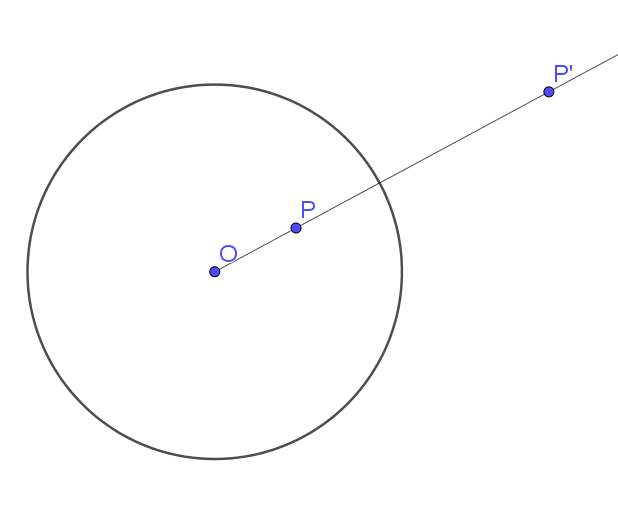
\includegraphics[width=0.6\linewidth]{inversion_definition}
	\label{fig:inversiondefinition}
\end{figure}

Just from this definition, we can start thinking about a few properties.
(Compare these properties to those of reflection over a line!)

\begin{itemize}
	\ii If $P$ is inside the circle, then $OP < r$, so $OP^\ast > r$,
	meaning $P^\ast$ is outside the circle (and vice versa).
	\ii The only points that don't move are the ones on $\omega$,
	since $OP = r \iff OP^\ast = r$.
	\ii $P$ and $P^\ast$ swap with each other, which means that
	reflecting about the same circle twice is equivalent to
	doing nothing. As a fun consequence, the converse of
	pretty much any statement you make will be true
	(this is a heuristic judgment, not a formal theorem).
\end{itemize}

At this point, you may have come across the thought, ``What happens to $O$?''
since $OO = 0$. To resolve this, we adjoin the ``point at infinity''
(denoted $\infty$) to the real plane, which we declare
to lie on every single line and be arbitrarily far away
from all the other points in the plane; then, we can say that
$O$ and $\infty$ swap.

\section{Preliminary properties}

The first thing that we should figure out is,
``How do I construct $P^\ast$ given $P$ and $\omega$?''
\begin{problem}
	Construct $P^\ast$.
\end{problem}

The only pieces of information we have are that $P^\ast$ lies on 
$\overrightarrow{OP}$ and $OP\cdot OP^\ast = r^2$.
The second condition can be rewritten as
\[\frac{OP}{r} = \frac{r}{OP^\ast},\]
so, really, this is signaling that we should be looking for similar triangles.
(In fact, any radius not collinear with $OP$ should generate
a pair of similar triangles --- prove this.)

If we draw the right radius, this becomes simple:

\begin{figure}[h]
	\centering
	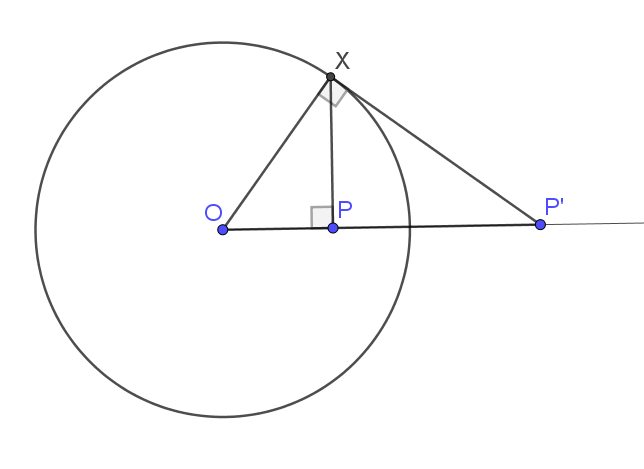
\includegraphics[width=0.7\linewidth]{inversion_construct}
	\label{fig:inversionconstruct}
\end{figure}

More precisely, $X$ is one of the intersections of $\omega$ and
the perpendicular to line $OP$ at $P$, and $P^\ast$ is
the intersection of $\overrightarrow{OP}$ with the perpendicular to
$OX$ at $X$. Then, $\triangle OPX\sim\triangle OXP^\ast$
gives the desired ratio relation.

\pagebreak

\begin{problem}
	If $A$ and $B$ are not collinear with $O$ and do not lie on $\omega$,
	show that quadrilateral $ABB^\ast A^\ast$ is cyclic.
\end{problem}

This is immediate by similar triangles --- feel free to work out the details.
The key idea is $\triangle OAB\sim\triangle OB^\ast A^\ast$.
(Often, the similar triangles more relevant than the fact that
the points are concyclic.)

\begin{figure}[h]
	\centering
	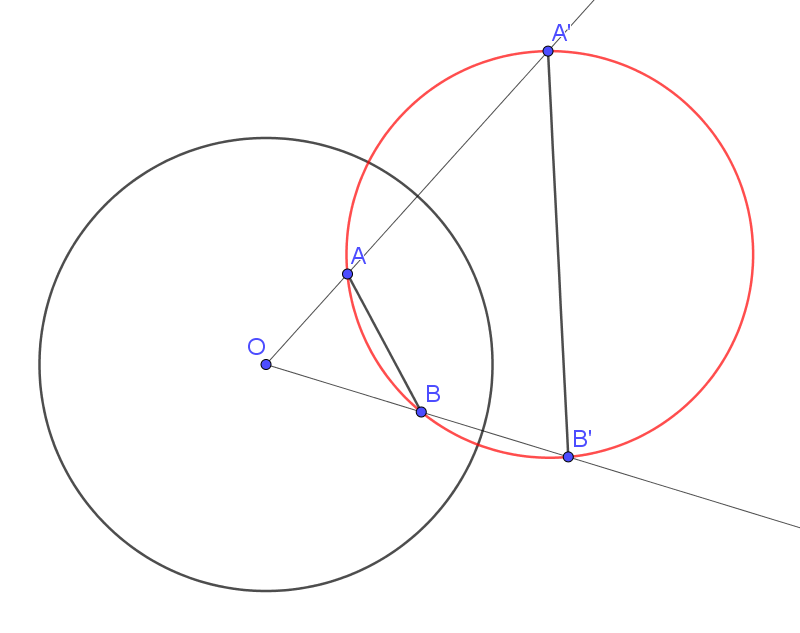
\includegraphics[width=0.7\linewidth]{inversion_cyclic}
	\caption{$\triangle OAB\sim\triangle OA^\ast B^\ast$.}
	\label{fig:inversioncyclic}
\end{figure}

\pagebreak

\section{Where do circles and lines go?}

In the previous section, we showed that,
if $A$, $B$, and $C$ are concyclic with $O$,
then $A^\ast$, $B^\ast $, and $C^\ast $ must be collinear, which means
\alert{that the circumcircle of $ABCO$ actually gets sent to a line}.
Conversely, \alert{lines not passing through $O$ map to circles through $O$}.

However, there are still some cases left: What if a line does go through $O$?
What about circles that don't pass through $O$?

\begin{theorem}[Images of circles and lines]
	Here is the full description of where circles and lines get sent
	under the transformation:
	\begin{enumerate}
		\ii The image of a line passing through $O$ is the same line.
		\ii The image of a line not passing through $O$
		is a circle passing through $O$, and vice versa.
		\ii The image of a circle not passing through $O$ is
		another circle not passing through $O$.
	\end{enumerate}
\end{theorem}

\begin{proof} We show each part separately:
\\

(1) Let $\ell$ be a line that contains $O$.
Obviously, each point on line $\ell$ gets sent to another point on $\ell$.
On the other hand, there are no ``holes'' in the image of $\ell$ because
the transformation swaps pairs of points $A$, $A^\ast $ satisfying $OA\cdot OA^\ast  = r^2$
(it might help to follow along with a discrete analog, say 10 points in a row).
This means that the entire line is ``preserved,''
despite the points on the line getting shuffled around.
\\

(2) Here's a second proof of the fact that circles through $O$ get sent to lines
(or rather, its converse).
Pick some line $\ell$ not passing through $O$, and let $P$ be
the foot of the altitude from $O$ to $\ell$. 

\begin{figure}[h]
	\centering
	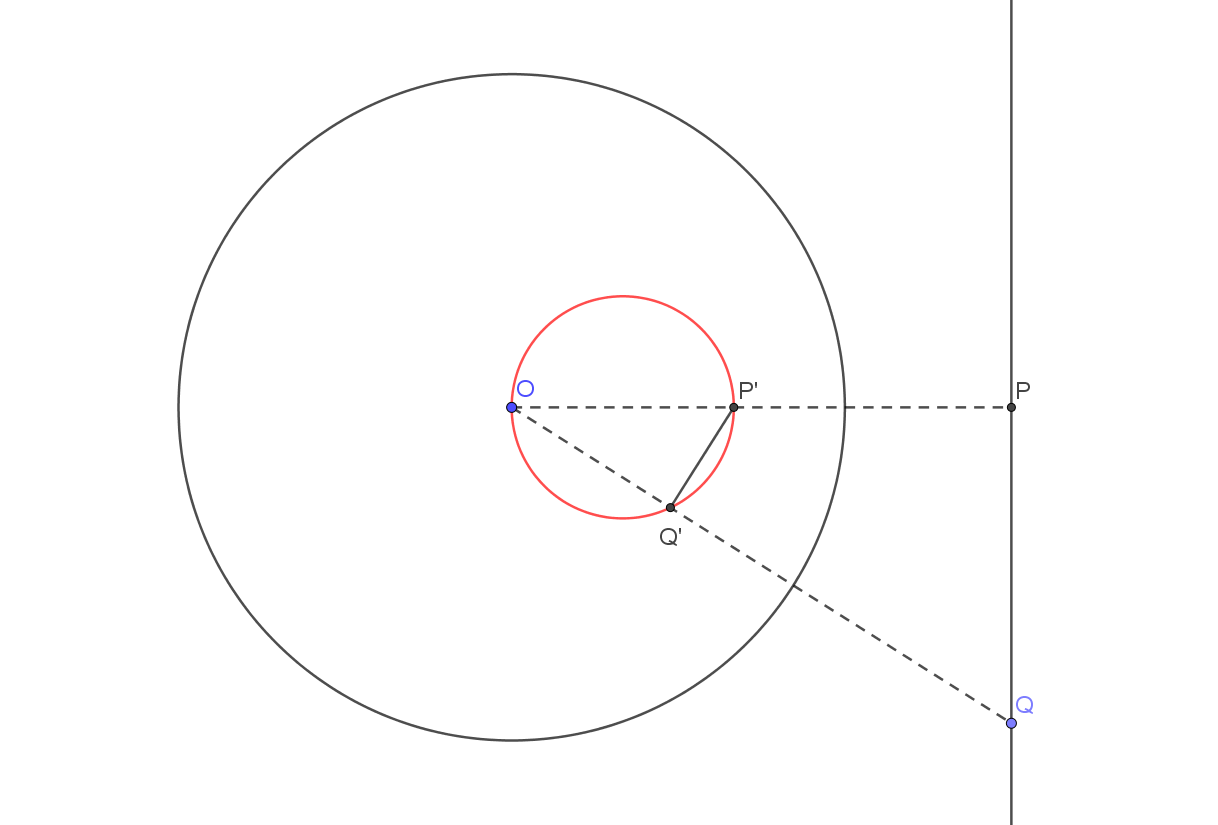
\includegraphics[width=0.8\linewidth]{inversion_circleToLine}
	\caption{Circles $\leftrightarrow$ lines!}
	\label{fig:inversioncircletoline}
\end{figure}

Then, $P$ gets sent to some $P^\ast $.
Now, arbitrarily choose a point $Q$ on $\ell$, and consider its image $Q^\ast $.
We know that
\[OP\cdot OP^\ast  = OQ\cdot OQ^\ast  = r^2\implies \frac{OQ}{OP} = \frac{OP^\ast }{OQ^\ast },\]
so $\triangle OPQ\sim\triangle OQ^\ast P^\ast $. In turn,
$\angle OQ^\ast P^\ast  = 90\dg$, regardless of $Q$: that is, $Q^\ast $ always lies on
the circle with diameter $OP^\ast $. Varying $Q$ across all points in $\ell$
in fact shows that every point on the circle is the image of
some point on $\ell$ (with the pre-image of $O$ being $\infty$).
\\

(3) The proof of this is extremely neat, in my opinion.

Let $ABDC$ be a cyclic quadrilateral
(sorry, I'm too lazy to change the order of the points in my GeoGebra diagram)
with circumcircle $\Gamma$,
and let $T$ be a tangent from $O$ to $\Gamma$. 

\begin{figure}[h]
	\centering
	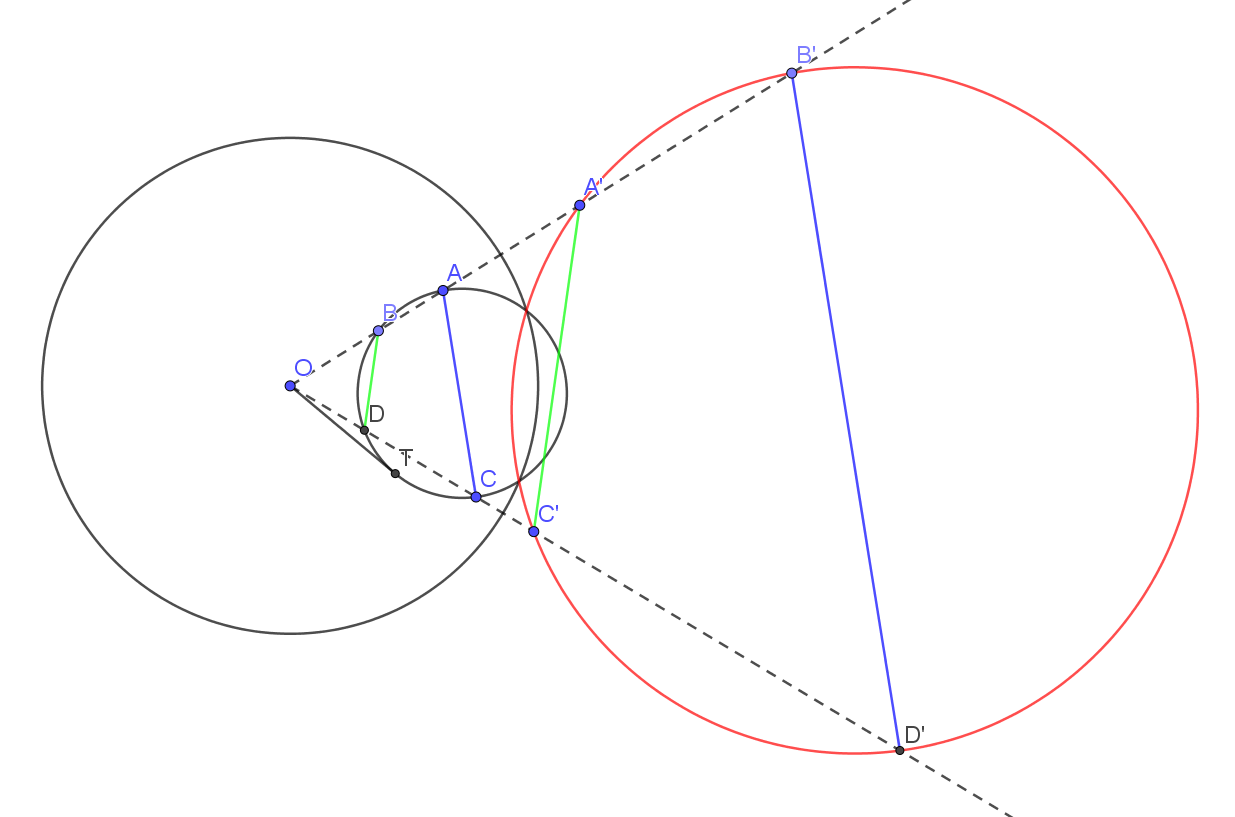
\includegraphics[width=0.75\linewidth]{inversion_circleToCircle}
	\caption{What do you know about segment $OT^\ast$?}
	\label{fig:inversioncircletocircle}
\end{figure}

Power of a point says
\[OA\cdot OB = OC\cdot OD = OT^2,\]
which tells us that
\[OA^\ast  = \frac{r^2}{OA} = \frac{r^2\cdot OB}{OA\cdot OB} =
\frac{r^2\cdot OB}{OT^2}\]
and the symmetric expressions. In particular, consider
$\triangle OBD$. We have
\[OA^\ast  = \frac{r^2}{OT^2}\cdot OB,\quad OC^\ast  = \frac{r^2}{OT^2}\cdot OD,\]
meaning $\triangle OA^\ast C^\ast $ is a dilation of $\triangle OBD$ with scale factor
$\frac{r^2}{OT^2}$. Similarly, $\triangle OB^\ast D^\ast $ is a dilation of
$\triangle OAC$ \emph{with the same scale factor}, so we get
the incredibly strong result that $A^\ast B^\ast D^\ast C^\ast $ is a dilation of $BACD$,
and thus their circumcircles must map to one another.
(Keen-eyed geometers may recognize the key idea of this proof as a variant on
\href{https://pleasantonmathcircle.org/assets/mat/CyclicQuad.pdf#page=3}
{Reim's theorem}.)

\noindent At this point, we have exhausted all the cases, so we are done!
\end{proof}

\begin{remark}[Small detail]
	When we say ``Shape $\mathcal S$ gets mapped to shape $\mathcal T$
	by transformation $f$,'' we mean that $f\colon\mathcal S\to\mathcal T$
	is bijective; in particular, $f$ need not send points to any specific location
	beyond ``from $\mathcal S$ to $\mathcal T$.''
	This becomes pretty important in the study of projective transformations,
	where things can be very hard to visualize due the generality of
	the transformations, but it's relevant here, too, as it allows us
	to formalize the notion of ``line $\ell$ gets sent to itself,'' for example.
\end{remark}

\begin{remark}[Note for experts]
	In the second part (where circles get sent to lines), it turns out that
	$\ell$ is the radical axis of $\omega$ and $\ell^\ast $ ---
	thanks to Andrew for pointing this out.
	Additionally, $\omega$, $\Gamma$, and $\Gamma^\ast $ are either
	coaxial or concentric in the third part.
\end{remark}

It's worth sketching a few images to get a sense of what they look like.
\begin{figure}[h]
	\centering
	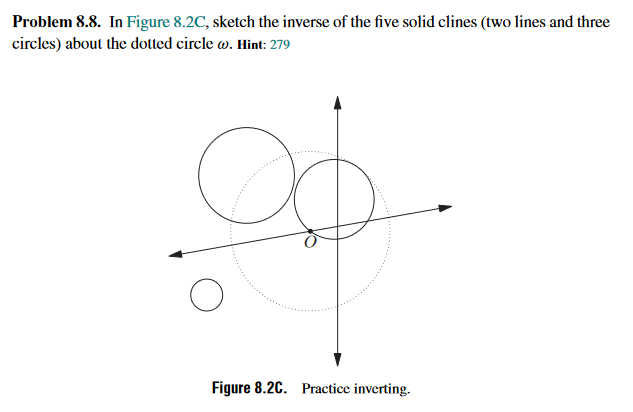
\includegraphics[width=0.7\linewidth]{inversion_egmo88}
	\caption{From \emph{Euclidean Geometry in Mathematical Olympiads}.}
	\label{fig:inversionegmo88}
\end{figure}

The upshot of all of this is that circles and lines are the same ``type of object,''
in some sense. In particular, this weird reflection allows you to
swap concyclicity for collinearity, lines for circles, and circles for lines.

\begin{quote}
	\emph
	{It is almost like you are given a choice---which of these two problems
	looks easier, the inverted one or the original one?
	Which would you like to solve?}
	
	\hfill{} Evan Chen, \emph{Euclidean Geometry in Mathematical Olympiads}
\end{quote}

\pagebreak

\section{Orthogonal circles}
\begin{problem}
	Given a circle $\Gamma$ and a point $O$, construct $\omega$
	such that $\Gamma^\ast  = \Gamma$.
\end{problem}

As we mentioned in class, an important property of the reflection is
the fact that points on $\omega$ stay where they are --- they are fixed points.
This fact is incredibly useful when drawing out the images of shapes
(e.g. the exercise above). You might gather, then, that having an entire
fixed circle would be extremely nice, which is what makes this a very
useful question to answer.

First, let's gather some observations.
\begin{itemize}
	\ii Circle $\Gamma$ cannot be entirely inside or entirely outside $\omega$,
	as reflection swaps inside and outside.
	\ii If $P$ and $Q$ are points on $\Gamma$ that are collinear with $O$,
	then $P$ and $Q$ must be each other's image.
	In particular, this means $Q = P^\ast $ and so
	\[OP\cdot OQ = OP\cdot OP^\ast  = r^2.\]
	\ii By power of a point, $OP\cdot OQ = OT^2 = r^2$
	where $OT$ is a tangent to $\Gamma$. This means the tangency points
	from $O$ to $\Gamma$ must lie on $\omega$.
\end{itemize}

Actually, we are now done: there is only one circle centered at $O$
passing through the tangency points from $O$ to $\Gamma$;
so there's our construction!

\begin{figure}[h]
	\centering
	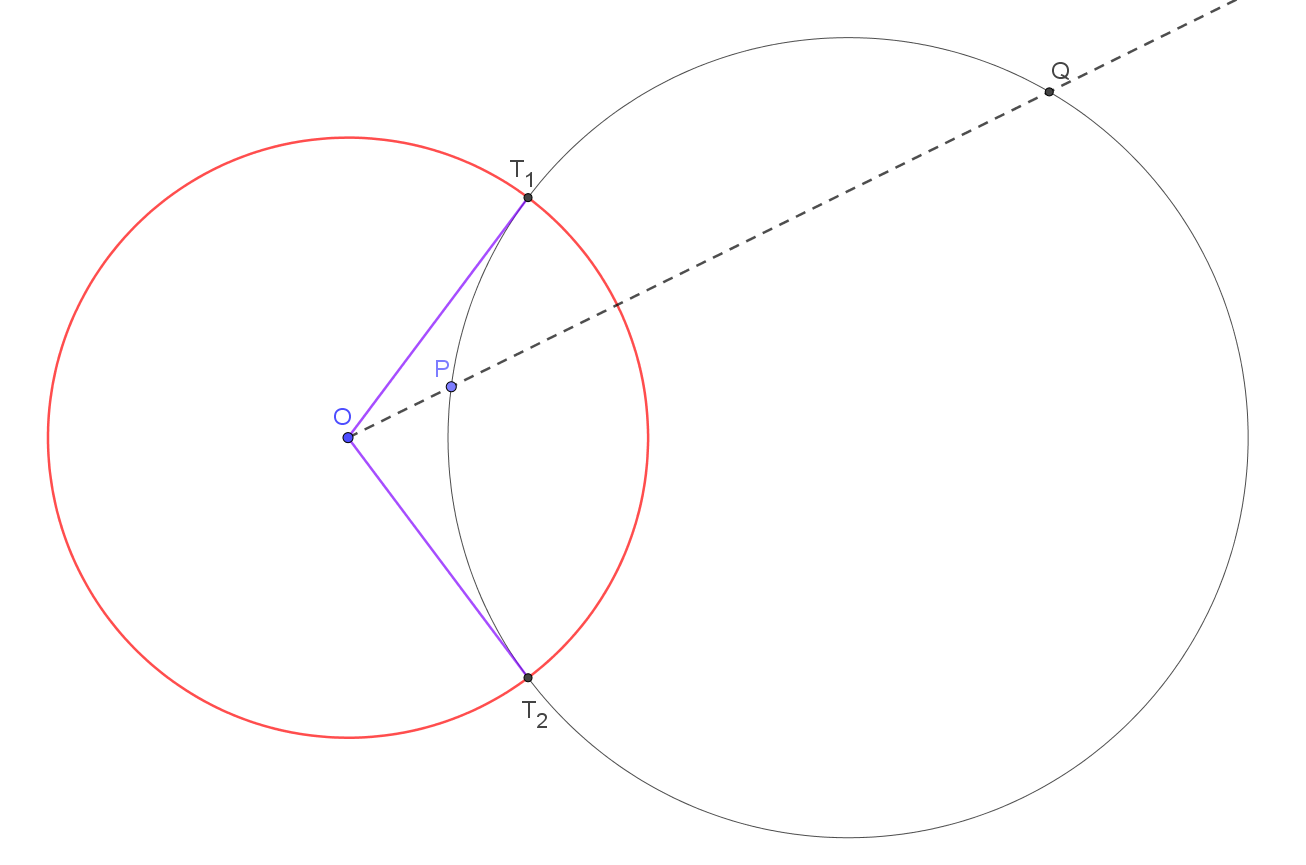
\includegraphics[width=0.7\linewidth]{inversion_orthogonal}
	\label{fig:inversionorthogonal}
\end{figure}

\begin{definition}
	Two circles $\omega_1$ and $\omega_2$ are \alert{orthogonal}
	if the image of $\omega_1$ upon reflection over $\omega_2$
	is $\omega_1$ (and vice versa).
\end{definition}

\begin{warning}
	The circle being preserved does not mean that special points
	are the same in the image. For example, the center of $\Gamma$
	swaps with the midpoint of $T_1T_2$.
\end{warning}

\begin{exercise}
	Suppose two orthogonal circles intersect at $T$.
	Show that the tangents to the circles at $T$ are perpendicular.
\end{exercise}

\begin{exercise}[Surprisingly useful!]
	Let two orthogonal circles $\omega_1$ and $\omega_2$ intersect at $T$,
	and let $\Gamma$ be a circle centered at $T$.
	Show that the images of $\omega_1$ and $\omega_2$
	upon reflection over $\Gamma$ are perpendicular.
\end{exercise}

\newpage
\section{Intersections}
Of course, normal geometry problems often have more than two
lines or circles.

\begin{theorem}
	Intersections between circles and lines are preserved by reflection.
\end{theorem}

The main point is that if, say, a circle and a line are tangent,
then they will be tangent after reflection, too ---
even if the line becomes a circle and the circle becomes a line.

These behave themselves in the nicest way possible:
the image of the intersection is the intersection of the images
(so, for a concrete example, two circles tangent at $O$
will map to two lines that intersect at $O^\ast = \infty$,
meaning the lines are parallel).

\section{Example problems}

\begin{problem}[Ptolemy's inequality]
	Given four points $A$, $B$, $C$, and $D$,
	\[AB\cdot CD + BC\cdot AD \ge AC\cdot BD,\]
	with equality if and only if $ABCD$ is convex and cyclic.
\end{problem}
\begin{proof}
	Let $\omega$ be a circle centered at $A$ with radius $r$,
	and reflect $B$, $C$, and $D$ about $\omega$.
	From Problem 2.2, we know that
	$\triangle ABC\sim\triangle AC^\ast B^\ast$,
	$\triangle ACD\sim\triangle AD^\ast C^\ast$, and
	$\triangle ADB\sim\triangle AB^\ast D^\ast$.
	In the former triangle,
	\[\frac{BC}{B^\ast C^\ast} = \frac{AB}{AC^\ast}
	\iff B^\ast C^\ast = \frac{AC^\ast}{AB}\cdot BC =
	\frac{AC\cdot AC^\ast}{AB\cdot AC}\cdot BC =
	\frac{r^2}{AB\cdot AC}\cdot BC.\]
	Analogously, we get
	\[C^\ast D^\ast = \frac{r^2}{AC\cdot AD}\cdot CD,\quad
	D^\ast B^\ast = \frac{r^2}{AD\cdot AB}\cdot DB.\]
	
	Then, the triangle inequality says
	\begin{align*}
		B^\ast C^\ast + C^\ast D^\ast &\ge B^\ast D^\ast\\
		\iff\frac{r^2}{AB\cdot AC}\cdot BC +
		\frac{r^2}{AC\cdot AD}\cdot CD &\ge
		\frac{r^2}{AD\cdot AB}\cdot DB\\
		\iff \frac{BC}{AB\cdot AC} + \frac{CD}{AC\cdot CD} &\ge
		\frac{DB}{AD\cdot AB}\\
		\iff BC\cdot AD + CD\cdot AB &\ge BD\cdot AC,
	\end{align*}
	with equality if and only if $B^\ast$, $C^\ast$, and $D^\ast$
	are collinear in that order.
	
	It then remains to show that $B^\ast$, $C^\ast$, and $D^\ast$
	are collinear if and only if $A$, $B$, $C$, and $D$ are concyclic
	in that order, which is as easy as observing
	\[180\dg = \angle AC^\ast B^\ast + \angle AC^\ast D^\ast =
	\angle ABC + \angle ADC\]
	meaning the equality case is indeed only when $ABCD$ is
	convex and cyclic.
\end{proof}

If anything, two things should be taken away from this proof:
one, that circles and lines swap under certain circumstances
(elaborated on in the next section), and two, that distances are often
easily computable by virtue of similar triangles.

\begin{problem}
	Let $\omega_1$, $\omega_2$, $\omega_3$, and $\omega_4$
	with consecutive pairs tangent at $A$, $B$, $C$, and $D$
	(so $\omega_1$ and $\omega_2$ are tangent at $A$, for example).
	Show that $A$, $B$, $C$, $D$ are either collinear or concyclic.
\end{problem}

\begin{figure}[h]
	\centering
	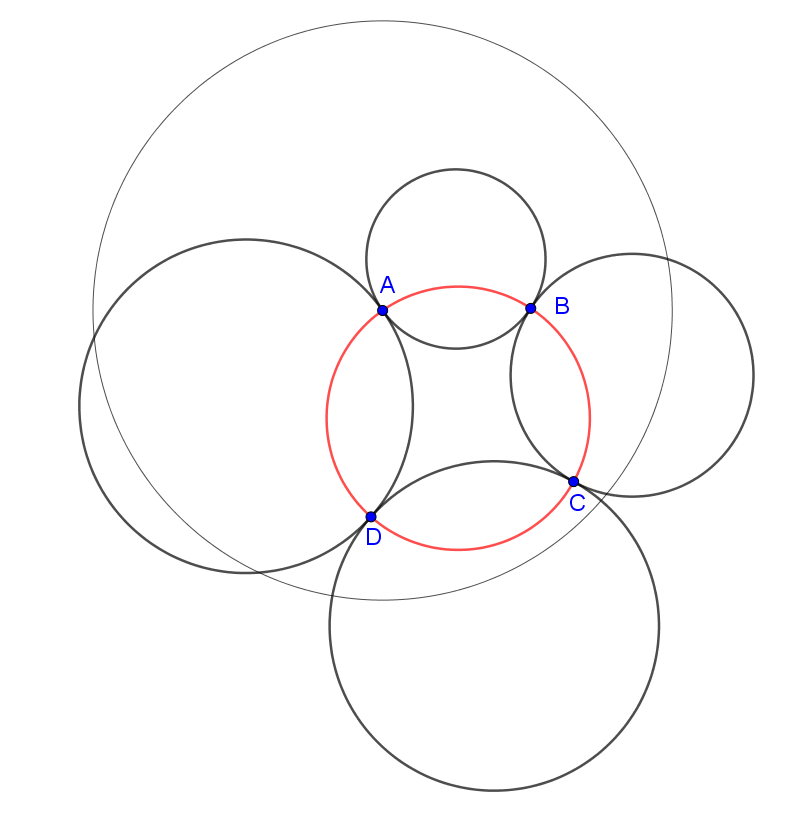
\includegraphics[width=0.5\linewidth]{inversion_egmo824}
	\label{fig:inversionegmo824}
\end{figure}

Let's reflect the picture over some circle centered at $A$
(the radius can be any positive real number your heart desires).
Try to follow along with a sketch of your own before looking at
the diagram on the next page!
\begin{itemize}
	\ii First, $\omega_1$ passes through $A$, so it gets sent to some line $\ell_1$.
	\ii Then, $\omega_4$ also passes through $A$ and is tangent to $\omega_1$,
	so it gets sent to some line parallel to $\ell_1$, say $\ell_4$.
	\ii Circles $\omega_2$ and $\omega_3$ become circles
	$\omega_2^\ast$ and $\omega_3^\ast$, which are tangent to both
	$\ell_1$ and $\ell_4$ at $B^\ast$ and $D^\ast$,
	as well as tangent to each other at $C^\ast$.
\end{itemize}
\pagebreak
\begin{figure}[h]
	\centering
	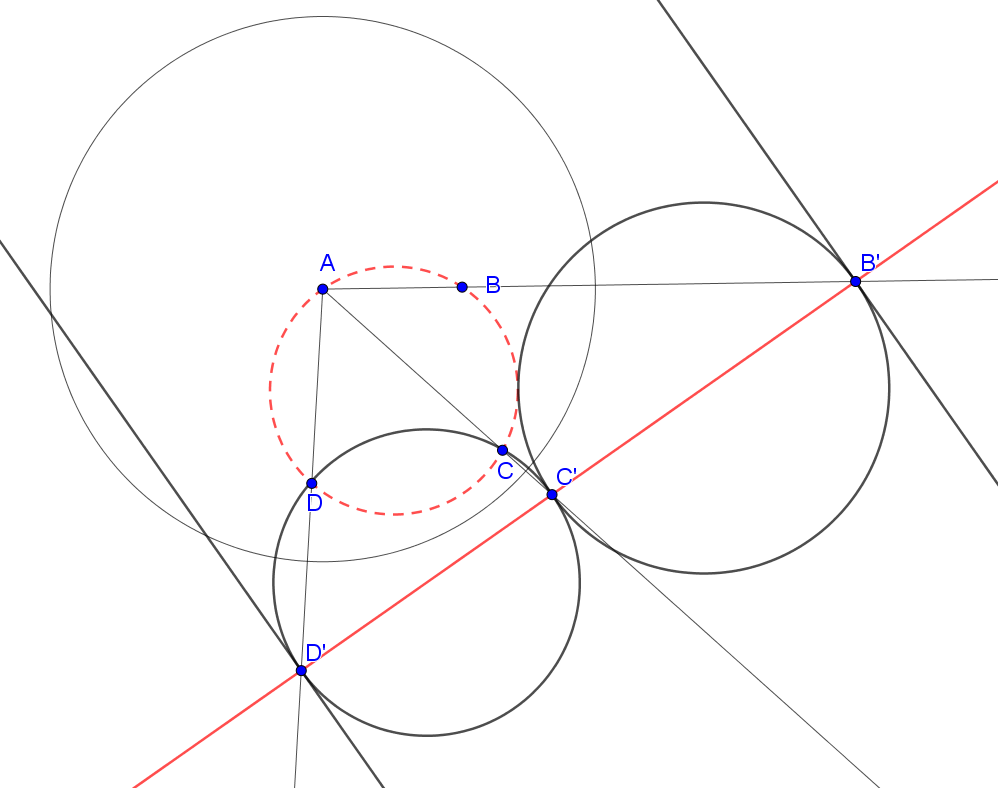
\includegraphics[width=0.7\linewidth]{inversion_egmo824img}
	\caption{The reflected picture, with most of the original diagram
	hidden away.}
	\label{fig:inversionegmo824img}
\end{figure}

Our goal now is to show that $B^\ast$, $C^\ast$, and $D^\ast$ are collinear.
Let $O_2$ and $O_3$ be the centers of $\omega_2^\ast$ and $\omega_3^\ast$.

\begin{figure}[h]
	\centering
	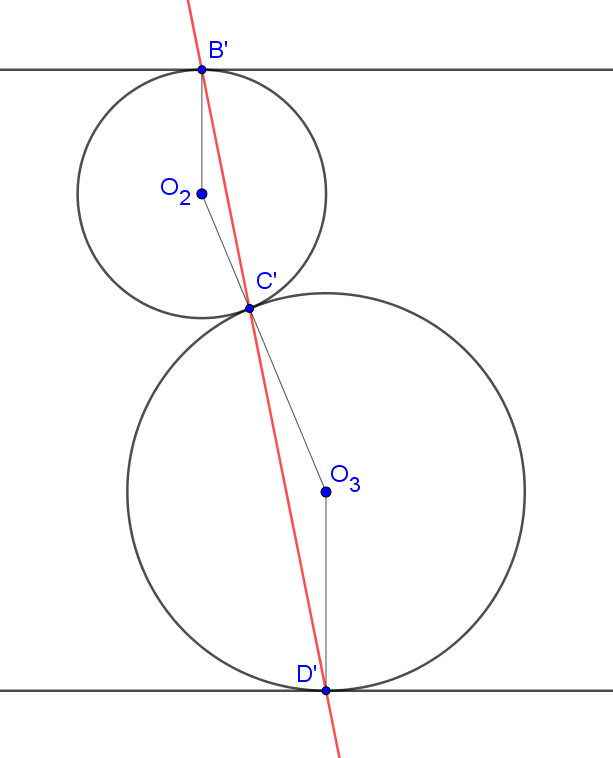
\includegraphics[width=0.4\linewidth]{inversion_egmo824img_focused}
	\label{fig:inversionegmo824imgfocused}
\end{figure}

Observe that $O_2B^\ast$ and $O_3D^\ast$ are parallel
since they are perpendicular to the parallel lines $\ell_1$ and $\ell_4$.
This tells us that
$\triangle B^\ast O_2C^\ast$ and $\triangle D^\ast O_3C^\ast$
are similar, so
\[\angle D^\ast C^\ast O_3 = \angle B^\ast C^\ast O_2 =
180\dg - \angle B^\ast C^\ast O_3\]
which implies the collinearity.

\begin{exercise}[Inspired by bad diagram]
	Determine when $B^\ast D^\ast$ is perpendicular to
	$\ell_1$ and $\ell_4$.
\end{exercise}

\pagebreak

\begin{problem}[Shortlist 1995 G3]
	In $\triangle ABC$, the incircle is tangent to $BC$, $CA$, and $AB$
	at $D$, $E$, and $F$ respectively.
	Point $X$ is chosen inside $\triangle ABC$ such that
	the incircle of $\triangle BCX$ is tangent to $BC$, $CX$, and $BX$
	at $D$, $Y$, and $Z$. Show that $E$, $F$, $Y$, and $Z$ are concyclic.
\end{problem}

This is an example of a problem that gets obliterated
once you choose the right circle to reflect about
and understand where everything goes.
Here's the diagram, for reference; try to draw the reflected objects
on your own, and make a conjecture about $E^\ast F^\ast Z^\ast Y^\ast$.

\begin{figure}[h]
	\centering
	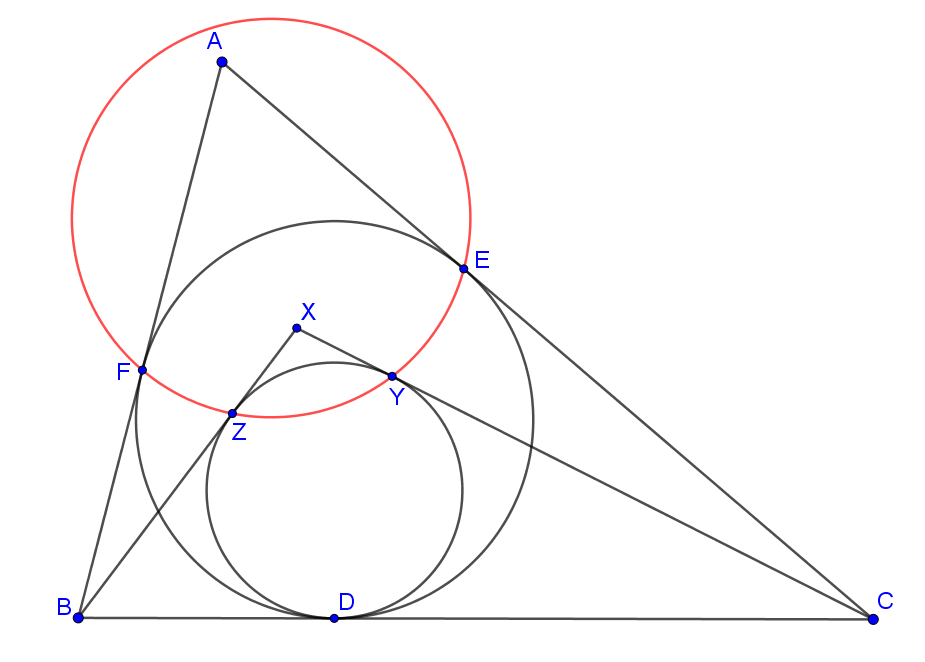
\includegraphics[width=0.7\linewidth]{inversion_twoIncircles}
	\label{fig:inversiontwoincircles}
\end{figure}

The main point is to center some circle $\omega$ at $D$
and reflect everything across $\omega$.

\paragraph{Solution 1 (9th grade geometry).}
This first solution uses nothing but angle chasing, actually.

\begin{figure}[h]
	\centering
	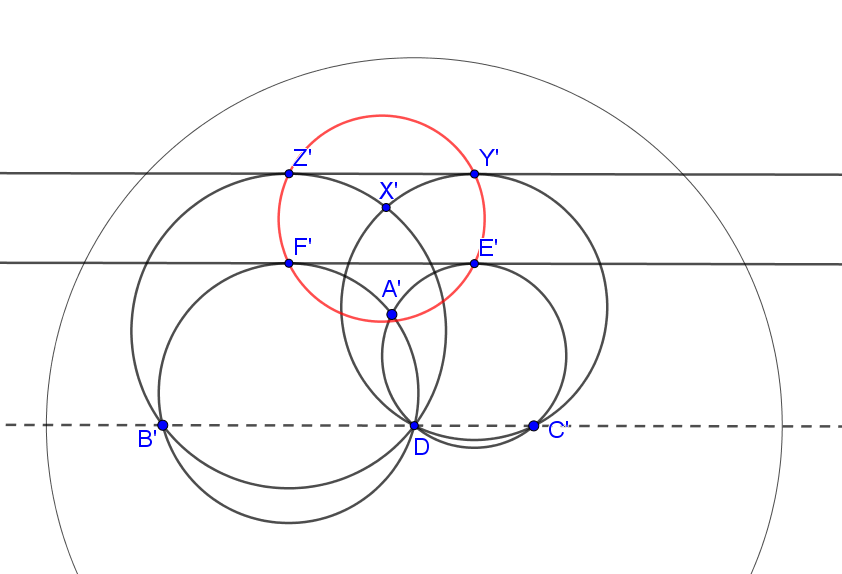
\includegraphics[width=0.7\linewidth]{inversion_twoIncircles_solution1}
	\label{fig:inversiontwoincirclessolution1}
\end{figure}

For the sake of comprehensiveness, the objects in the above picture
are related in the following ways:
\begin{enumerate}
	\ii Lines $B^\ast C^\ast$, $E^\ast F^\ast$, and $Y^\ast Z^\ast$ are parallel.
	\ii The circumcircles of $\triangle B^\ast DF^\ast$ and
	$C^\ast DE^\ast$ are tangent to line $E^\ast F^\ast$.
	\ii Similarly, the circumcircles of $\triangle B^\ast DZ^\ast$ and
	$C^\ast DY^\ast$ are tangent to line $Y^\ast Z^\ast$.
\end{enumerate}

The main mechanism for the solution is then to recognize the following:
\begin{claim}
	Triangles $\triangle B^\ast DF^\ast$, $C^\ast DE^\ast$,
	$B^\ast DZ^\ast$, and $C^\ast DY^\ast$ are all isosceles,
	with their bases on line $B^\ast C^\ast$.
\end{claim}
\begin{proof}
	This is just angle chasing. We prove the claim for
	$\triangle B^\ast DF^\ast$; the other three triangles
	follow the exact same logic.
	In particular,
	\[\angle DF^\ast E^\ast = \angle F^\ast DB^\ast\]
	by parallel lines, and
	\[\angle DF^\ast E^\ast = \angle F^\ast B^\ast D\]
	because of the tangency, directly giving the isosceles triangle.
\end{proof}

To finish, $F^\ast$ and $Z^\ast$ lie on the perpendicular bisector of
$B^\ast D$, meaning
$\angle Z^\ast F^\ast E^\ast = \angle F^\ast Z^\ast Y^\ast = 90\dg$.
Similarly,
$\angle Y^\ast E^\ast F^\ast = \angle E^\ast Y^\ast Z^\ast = 90\dg$,
too, so $E^\ast F^\ast Z^\ast Y^\ast$ is a rectangle, and thus cyclic!

\paragraph{Solution 2 (orthogonal circles).} The main mechanism
for this solution is Exercise 4.5.

\begin{figure}[h]
	\centering
	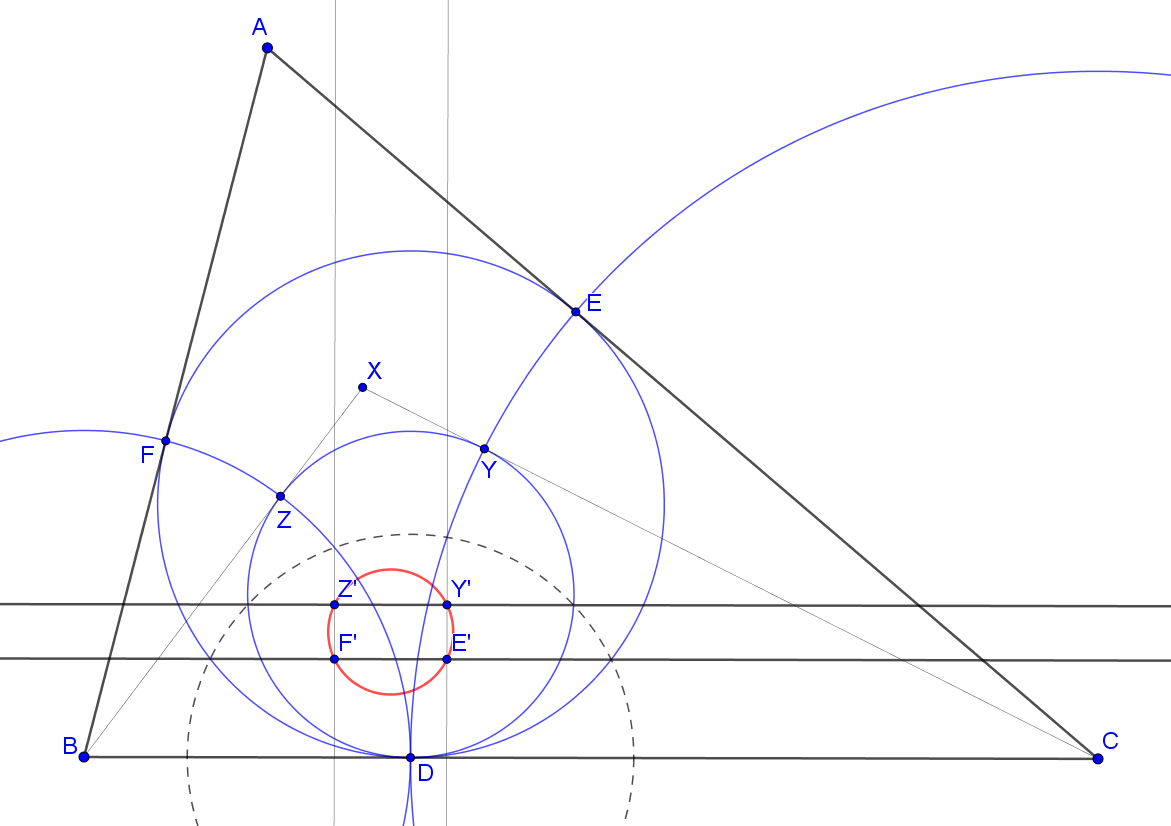
\includegraphics[width=0.8\linewidth]{inversion_twoIncircles_solution2}
	\caption{Secret orthogonal circles.}
	\label{fig:inversiontwoincirclessolution2}
\end{figure}

In particular, once you notice that $E^\ast F^\ast Z^\ast Y^\ast$
seems to be a rectangle, you should realize that there must be
a pair of orthogonal circles in the pre-image for each right angle.
Moreover, the relevant circles, which are marked blue in the diagram,
are precisely the pre-images of the sides of the rectangle.

This means that $(DFZ)$ (meaning ``the circumcircle of $\triangle DFZ$'')
and $(DEF)$ should be orthogonal, for example.
But this is obvious by construction, as $(DFZ)$ is the circle
centered at $B$ with radius $BD$ (prove it, if it isn't apparent).

Going backwards, the orthogonal circles immediately yield the right angles
and therefore the conjectured rectangle.
(I did call Exercise 4.5 ``surprisingly useful,'' right?)

\pagebreak

\section{Overlapping diagrams}
So far, our general strategy has been ``Let's reflect the entire diagram,
and, in the process, generate an entirely new problem
that we can solve separately.''
As a consequence, all of the problems in the previous section
only cared about the center of the circle of reflection.
This, however, loses a key piece of information about the transformation,
namely the radius associated with it.
Moreover, it completely ignores the original structure of the problem.

This section is thus dedicated to using this information
via choosing your circles to make pre-images and images interact cleanly.

\begin{problem}[Shoemaker's knife]
	Let $\Gamma$ be a semicircle with diameter $AB$ and
	let $C$ be a point on segment $AB$ that lies closer to $B$ than $A$.
	Define $\Omega$ to be the semicircle contained in $\Gamma$
	with diameter $AC$.
	Then, define the sequence of circles $(\omega_k)$
	such that $\omega_0$ has diameter $BC$ and, for $k > 0$,
	$\omega_k$ is tangent to $\omega_{k-1}$, $\Omega$, and $\Gamma$.
	
	Prove that the distance from the center of $\omega_n$ to $AB$ is
	$n$ times the diameter of $\omega_n$.
\end{problem}

There are so many circles here that it would be a crime not to invert.
\begin{exercise}
	Guess the center of the reflection, and reflect the diagram
	about an arbitrary circle centered at this point.
	What happens?
\end{exercise}

\begin{figure}[h]
	\centering
	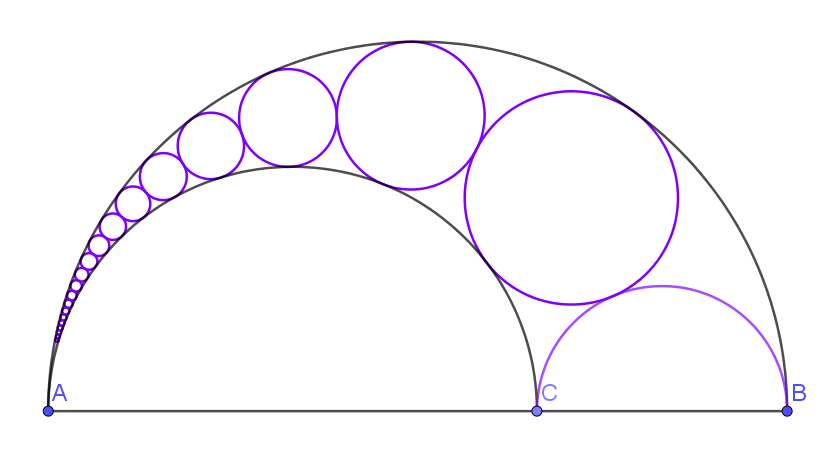
\includegraphics[width=0.7\linewidth]{shoemaker_diagram}
	\caption{This configuration is called a Pappus chain embedded in a shoemaker's knife.}
	\label{fig:shoemakerdiagram}
\end{figure}


Reflecting about a circle centered at $A$ sends
$\Gamma$ and $\Omega$ to some parallel lines,
and then, since each of the $\omega_i$ is tangent to
both circles and the previous circle, they transform into
a chain of congruent circles, with $\omega_0$ becoming a semicircle
centered on line $AB$.

\begin{figure}[h]
	\centering
	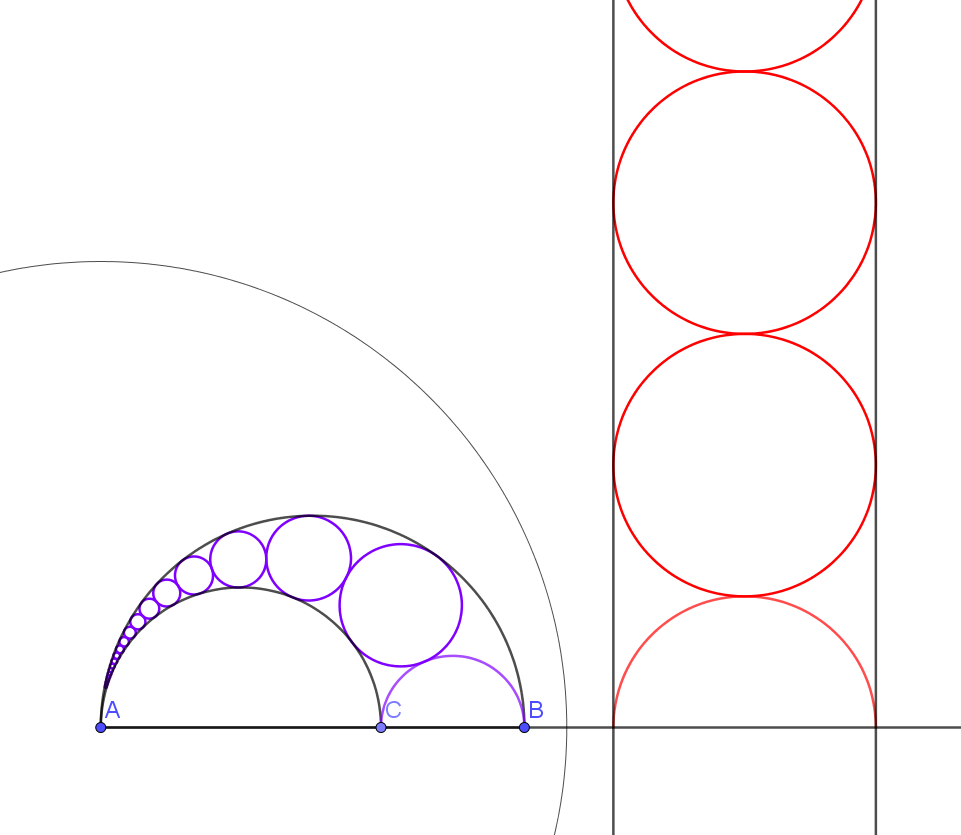
\includegraphics[width=0.7\linewidth]{shoemaker_inverted}
	\caption{All the circles in the chain become congruent!}
	\label{fig:shoemakerinverted}
\end{figure}

\pagebreak
However, the issue is that makes the information about
the radius of $\omega_k$ a lot less tractable, since any
relevant calculations would feature the arbitrary
radius of inversion heavily.
While this can eventually lead to a solution, we can do better.

The key trick is to preserve the radius of $\omega_k$.
We have a natural mechanism for preserving radii under inversion
using orthogonal circles, in fact.
Thus, the circle about which we are reflecting is
the circle centered at $A$ orthogonal to $\omega_k$.

\begin{figure}[h]
	\centering
	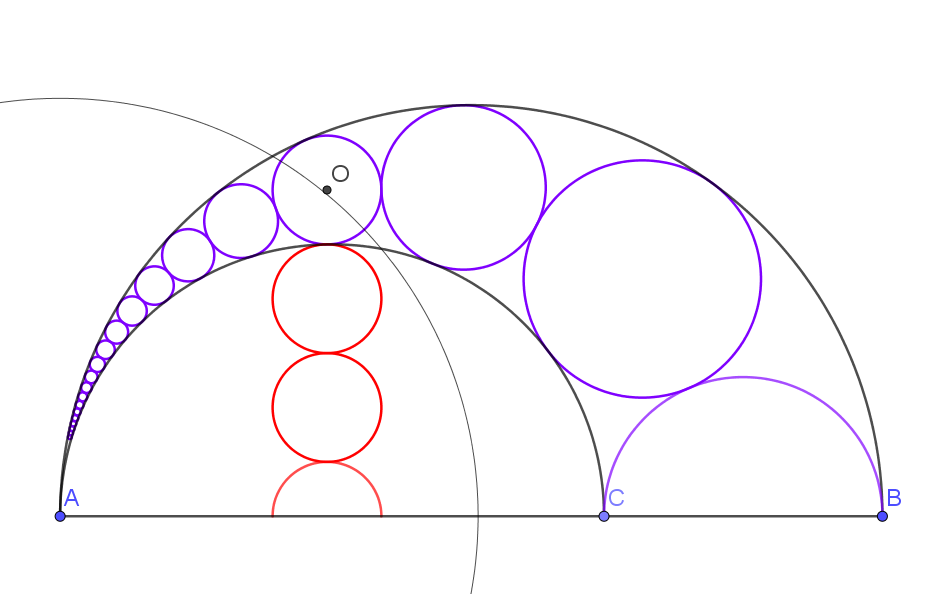
\includegraphics[width=0.7\linewidth]{shoemaker_overlaid}
	\caption{We have forced $\omega_3$ to map to itself here.}
	\label{fig:shoemakeroverlaid}
\end{figure}

This in fact gives us the result immediately ---
just look at the diagram!

\pagebreak

Often, a picture is centered about a triangle $ABC$,
in which case we don't want to offhandedly discard information
about the vertices. Here, we can use a composition of an inversion and
a line reflection cleverly to swap $B$ and $C$.

\begin{lemma}[Force-Overlaid Inversion]
	Let $\triangle ABC$ be a triangle. Then, inverting about $A$
	with radius $\sqrt{AB\cdot AC}$ followed by
	reflecting over the bisector of $\angle BAC$
	swaps $B$ and $C$.
\end{lemma}

\begin{problem}[Russian Olympiad 2009]
	In triangle $ABC$ with circumcircle $\Omega$, the internal angle bisector
	of $\angle A$ meets $BC$ at $D$ and $\Omega$ again at $E$.
	The circle with diameter $DE$ meets $\Omega$ again at $F$.
	Prove that $AF$ is a symmedian of triangle $ABC$.
\end{problem}

First, we define a symmedian:
\begin{definition}
	The $A$-symmedian of $\triangle ABC$ is the reflection of
	the $A$-median over the angle bisector of $\triangle ABC$.
\end{definition}

This means we should of course introduce the midpoint $M$ of $BC$.
Moreover, it turns out that $M$ lies on the circle $\Gamma$ with diameter $DE$
(why?), so the force-overlaid inversion should actually swap $M$ and $F$.

\begin{figure}[h]
	\centering
	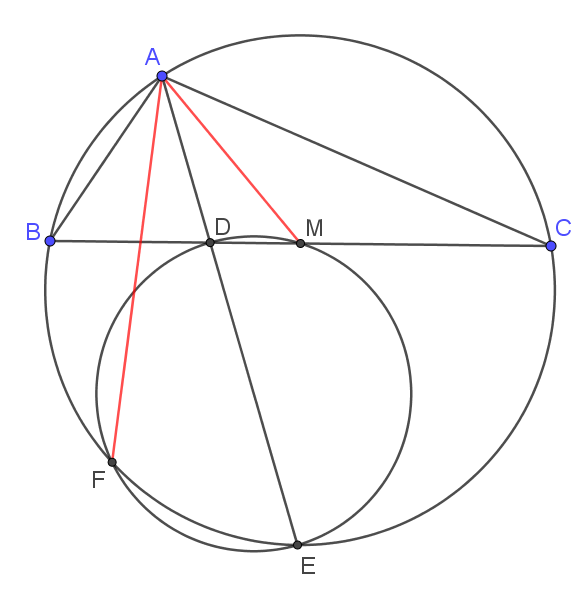
\includegraphics[width=0.6\linewidth]{rus2009_1}
	\caption{Lines $AM$ and $AF$ should be symmetric about $AE$.}
	\label{fig:rus20091}
\end{figure}

From $\triangle ABD\sim\triangle AEC$, we get
\[\frac{AB}{AD} = \frac{AE}{AC}\iff AB\cdot AC = AD\cdot AE,\]
so $D$ and $E$ get swapped, meaning the circle with diameter $DE$ is fixed.
Also, line $BC$ gets sent to the circumcircle of $AC^\ast B^\ast$,
which is just the circumcircle of $ABC$ since $(B, C) = (C^\ast, B^\ast)$.

Putting all this together means that the intersection of $BC$ and
the circle with diameter $DE$ gets sent to
the second intersection of $\Omega$ and the circle with diameter $DE$ ---
that is, $M$ gets sent to $F$ as desired.

\begin{exercise}
	Obliterate
	\href{https://artofproblemsolving.com/wiki/index.php/2012_AIME_II_Problems}
	{AIME II 2012/15}.
\end{exercise}


\pagebreak

\section{Practice problems}

\begin{problem}[By me!]
	Circles $\omega_1$, $\omega_2$, $\omega_3$, and $\omega_4$
	all pass through point $P$, with $\omega_1$ and $\omega_3$
	being tangent as well as $\omega_2$ and $\omega_4$.
	Moreover, the tangents to $\omega_1$ and $\omega_2$ at $P$
	are perpendicular,
	and $\omega_i$ and $\omega_{i+1}$ intersect at $X_i$, where
	$i = 1$, 2, 3, 4 and $\omega_5 = \omega_1$.
	If $PX_1 = 2$, $PX_2 = 6$, and $PX_3 = 3$, what is $PX_4$?
\end{problem}

\begin{problem}[AMC 12A 2017/16]
	Semicircles with centers at $A$ and $B$ and with radii 2 and 1,
	respectively, are drawn in the interior of, and sharing bases with, a
	semicircle with diameter $JK$. The two smaller semicircles are externally
	tangent to each other and internally tangent to the largest semicircle. A
	circle centered at $P$ is drawn externally tangent to the two smaller
	semicircles and internally tangent to the largest semicircle. What is the
	radius of the circle centered at $P$?
\end{problem}

\begin{problem}[USAMO 1993/2]
	Let $ABCD$ be a quadrilateral whose diagonals $AC$ and $BD$
	are perpendicular and intersect at $E$.
	Prove that the reflections of $E$ across
	$AB$, $BC$, $CD$, and $DA$ are concyclic.
\end{problem}

\begin{problem}[\emph{Euclidean Geometry in Mathematical Olympiads}, Problem 8.23]
	Let $ABC$ be a right triangle with $\angle C = 90\dg$
	and let $X$ and $Y$ be points in the interiors of $CA$ and $CB$,
	respectively. Construct four circles passing through $C$, centered
	at $A$, $B$, $X$, $Y$.
	Prove that the four points lying on exactly two of these four circles
	are concyclic.
\end{problem}

\begin{problem}[Brocard's theorem]
	Let $ABCD$ be a cyclic quadrilateral with circumcenter $O$.
	Define $P$ to be the intersection of $AB$ and $CD$,
	$Q$ to be the intersection of $AC$ and $BD$,
	and $R$ to be intersection of $AD$ and $BC$.
	Show that $O$ is the orthocenter of $\triangle PQR$.
\end{problem}

\begin{definition*}
	Let $P\ne O$ be a point in the plane. Then, the \alert{polar of $P$
	with respect to $\omega$} is the line through $P^\ast$
	perpendicular to line $OP$.
\end{definition*}

\begin{problem}
	Show that, if $P$ lies on the polar of $Q$, then
	the circle with diameter $PQ$ is orthogonal to $\omega$.
\end{problem}

\begin{problem}[Circles inscribed in segments]
	Let $BC$ be a chord of circle $\Omega$.
	Let $\omega$ be a circle tangent to $BC$ at $K$
	and internally tangent to $\omega$ at $T$.
	Show that
	\begin{itemize}
		\ii ray $TK$ passes through $M$, and
		\ii the power of $M$ with respect to $\omega$ is $MC^2$
		(that is, $MT\cdot MK = MC^2$).
	\end{itemize}
\end{problem}

\begin{problem}[Shortlist 2003 G4]
	Let $\Gamma_1$, $\Gamma_2$, $\Gamma_3$, $\Gamma_4$ be
	distinct circles such that $\Gamma_1$, $\Gamma_3$
	are externally tangent at $P$ and $\Gamma_1$, $\Gamma_1$
	are externally tangent at the same point $P$.
	Suppose that $\Gamma_1$ and $\Gamma_2$, $\Gamma_2$ and $\Gamma_3$,
	$\Gamma_3$ and $\Gamma_4$, $\Gamma_4$ and $\Gamma_1$ meet at
	$A$, $B$, $C$, $D$, respectively.
	Prove that
	\[\frac{AB\cdot BC}{AD\cdot DC} = \frac{PB^2}{PD^2}\]
\end{problem}

\end{document}